\documentclass[12pt,a4paper]{article}

\usepackage{amsmath}
\usepackage{palatino}
\usepackage{lipsum}
\usepackage{mwe}
\usepackage{graphicx}
\usepackage{tabularx}
\usepackage{color}
\usepackage{amssymb}
\usepackage{float}
\usepackage{amsfonts}
\usepackage{subfigure}
\usepackage{apacite}
\usepackage{fullpage}
\usepackage{bm}


\begin{document}
\thispagestyle{empty}
\Large \textbf{Part \uppercase\expandafter{\romannumeral2} - Generating Mosaics}

~\\
\normalsize \textbf{Task 1}\\ 
\par We can formulate the mosaic generation task as a linear problem with binary constraints.
\begin{equation*}
\begin{aligned}
min_{x}\indent& \sum_{k=1}^{r}\sum_{j=1}^{n}\sum_{i=1}^{m}(c_{k}-\beta_{i,j})^{2}x_{i,j,k}\\
s.t.\indent& \sum_{k=1}^{r}x_{i,j,k}=1, \forall i,j\\
& \sum_{j=1}^{n}\sum_{i=1}^{m}x_{i,j,k}=t, \forall k\\
&  x_{i,j,k} \in \{0,1\}, \forall i,j,k
\end{aligned}
\end{equation*}		
Note that $t=(\frac{m}{l}\cdot\frac{n}{l})/r$, which is the times of each tile being used.\\
\indent Since the task requires us to solve the linear program via the simplex method, then we transform the above problem again.
\begin{equation*}
\begin{aligned}
min_{\textbf{x}}\indent& c^{T}\textbf{x}\\
s.t.\indent& A\textbf{x}=b\\
& x_{i,j,k} \in [0,1], \forall x_{i,j,k}\in \textbf{x}\\
\end{aligned}
\end{equation*}	
Note that we transform all the $x_{i,j,k}$ into a column vector \textbf{x}, and make the objective function as $c^{T}\textbf{x}$, the constraints as $A\textbf{x}=b$. In details, here $\textbf{x} = [x_{1,1,1},\cdots,x_{r,1,1},x_{1,1,2},\cdots,$\\
$x_{r,1,2},\cdots,x_{1,m,n},\cdots,x_{r,m,n}]^{T}$. $A$ contains 0 and 1 in certain regular, $b$ contains $1$ for $m\cdot n$ times and $t$ for $r$ times. Also, we relax binary $x$ to $x_{i,j,k} \in [0,1]$.\\
\par Then we use \textit{linprog} in MATLAB to solve the linear program. Here we apply 3 kinds of figures and 2 kinds of tiles to conduct the mosaic task.\\
\indent The results of mosaic task are as following. Figure 2,5,8 apply 40*40 circle tiles to generate mosaics. Figure 3,6,9 apply 64*64 symbol tiles to generate mosaics.
\begin{figure}[htbp]
\centering
\begin{minipage}[t]{0.32\linewidth}
	\centering
	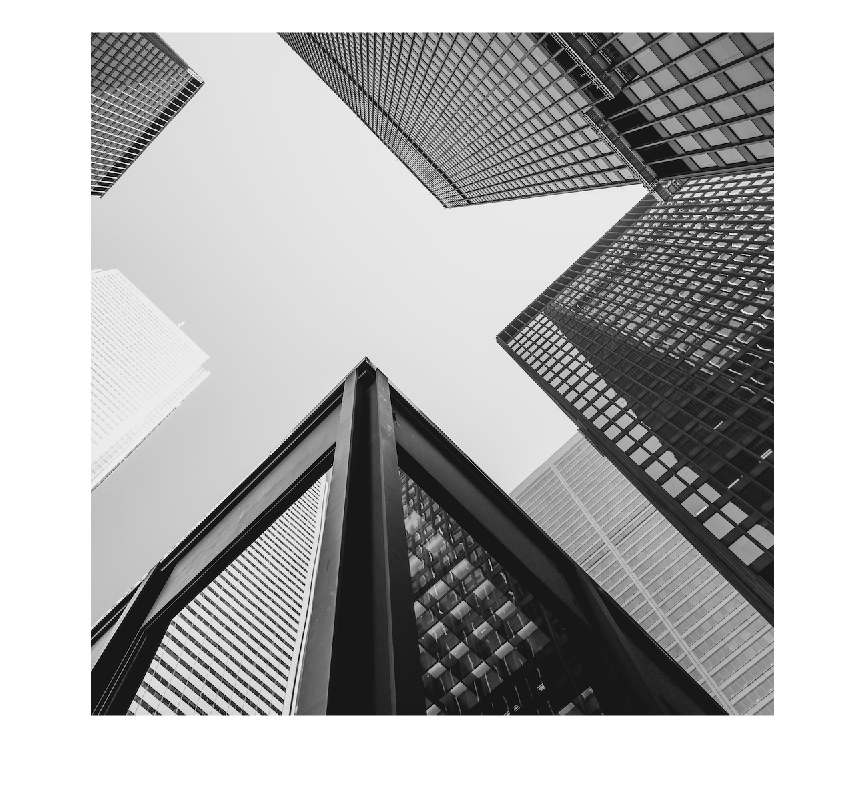
\includegraphics[width=5cm,height=5cm]{city_gray.png}
	\caption{City Gray}
\end{minipage}
\begin{minipage}[t]{0.32\linewidth}
	\centering
	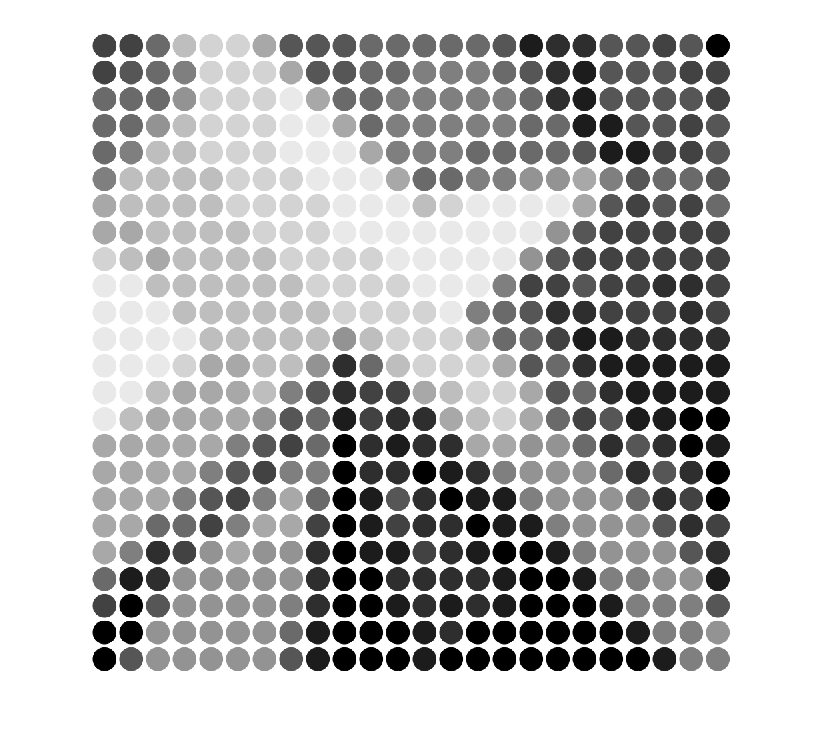
\includegraphics[width=5cm,height=5cm]{city_circle_40.png}
	\caption{City Circle}
\end{minipage}
\begin{minipage}[t]{0.32\linewidth}
	\centering
	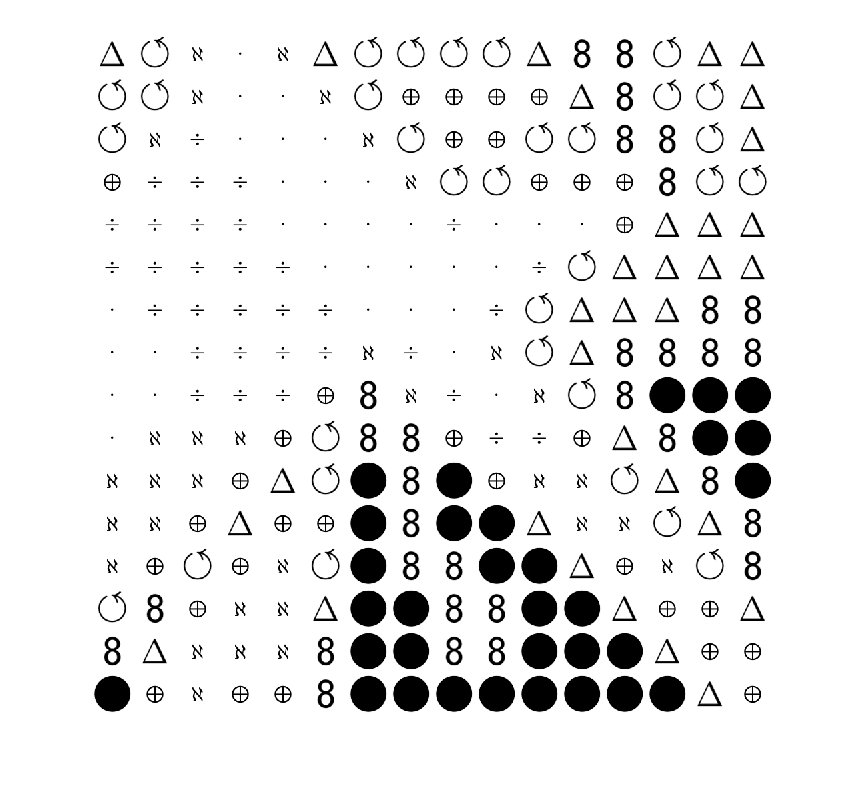
\includegraphics[width=5cm,height=5cm]{city_symbol_64.png}
	\caption{City Symbol}
\end{minipage}                        
\end{figure}	

\newpage
\thispagestyle{empty}	
\begin{figure}[htbp]
	\centering
	\begin{minipage}[t]{0.32\linewidth}
		\centering
		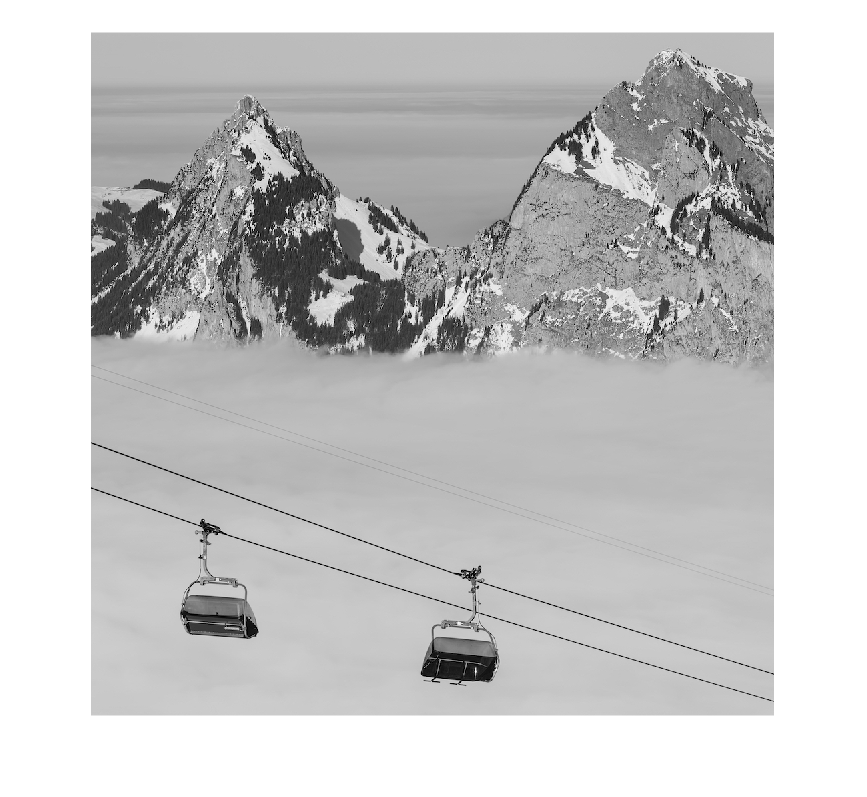
\includegraphics[width=5cm,height=5cm]{mountain_gray.png}
		\caption{Mountain Gray}
	\end{minipage}
	\begin{minipage}[t]{0.32\linewidth}
		\centering
		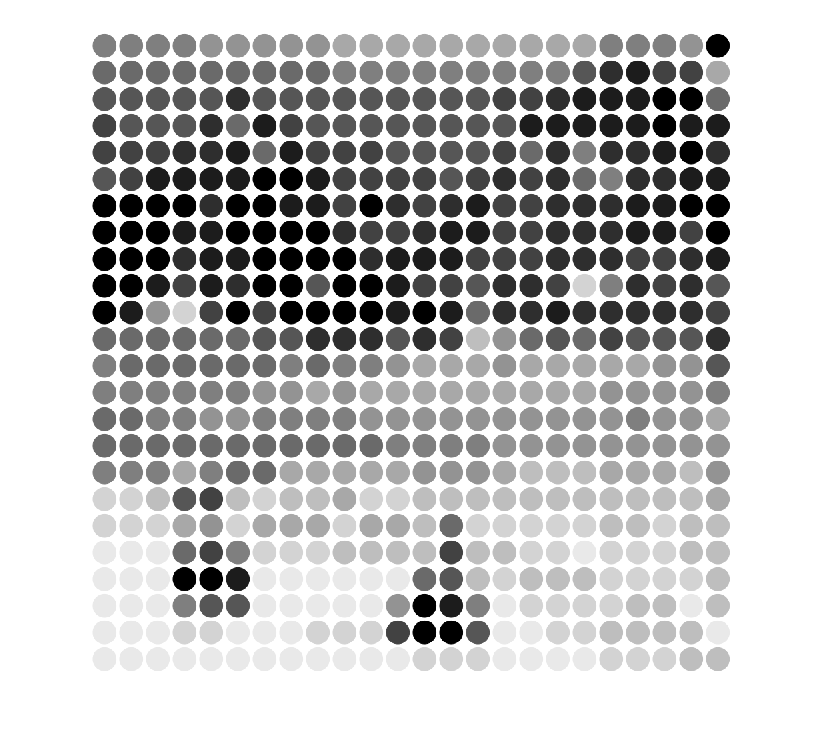
\includegraphics[width=5cm,height=5cm]{mountain_circle_40.png}
		\caption{Mountain Circle}
	\end{minipage}
	\begin{minipage}[t]{0.32\linewidth}
		\centering
		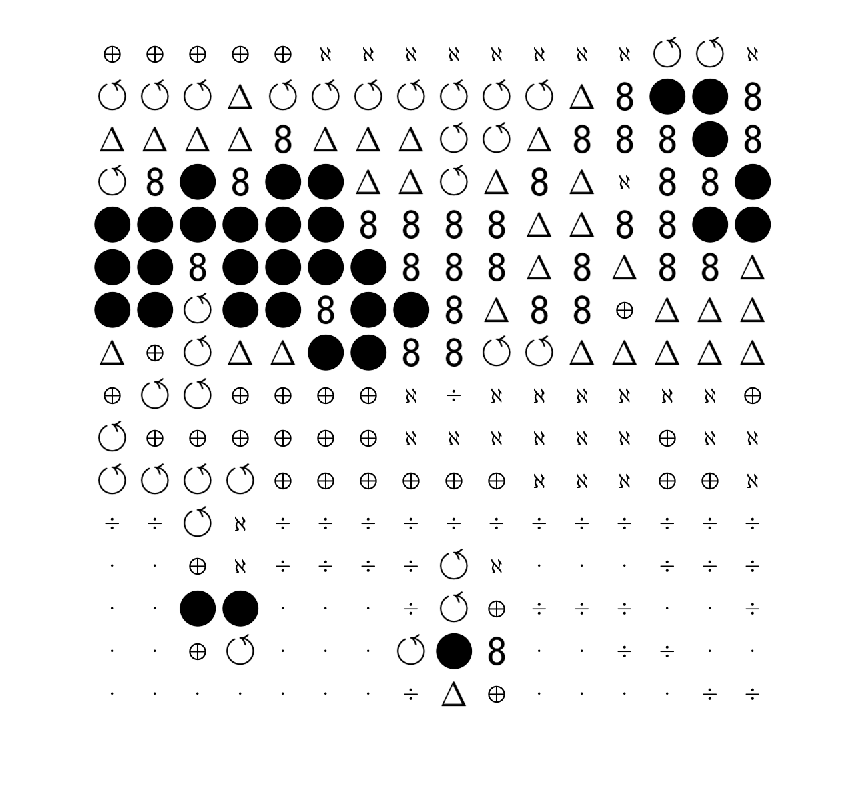
\includegraphics[width=5cm,height=5cm]{mountain_symbol_64.png}
		\caption{Mountain Symbol}
	\end{minipage}                        
\end{figure}		

\begin{figure}[htbp]
	\centering
	\begin{minipage}[t]{0.32\linewidth}
		\centering
		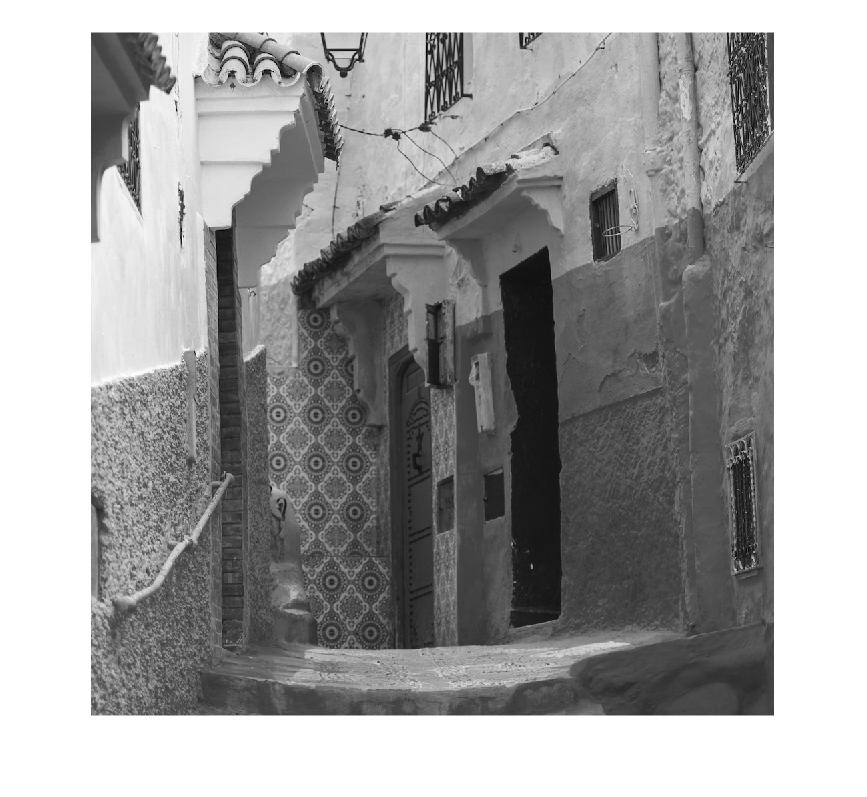
\includegraphics[width=5cm,height=5cm]{bluestreet_gray.png}
		\caption{Street Gray}
	\end{minipage}
	\begin{minipage}[t]{0.32\linewidth}
		\centering
		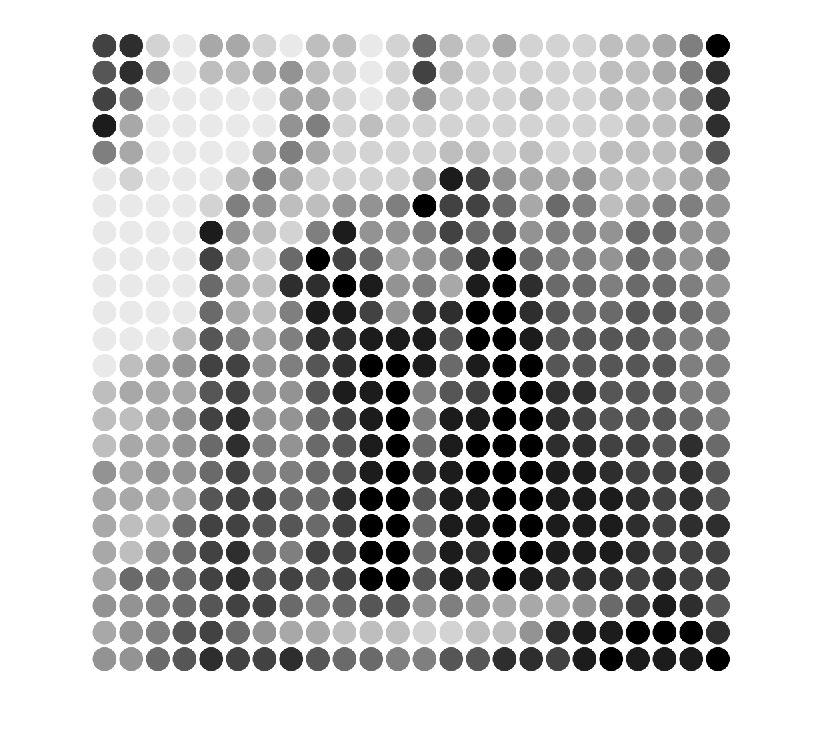
\includegraphics[width=5cm,height=5cm]{bluestreet_circle_40.png}
		\caption{Street Circle}
	\end{minipage}
	\begin{minipage}[t]{0.32\linewidth}
		\centering
		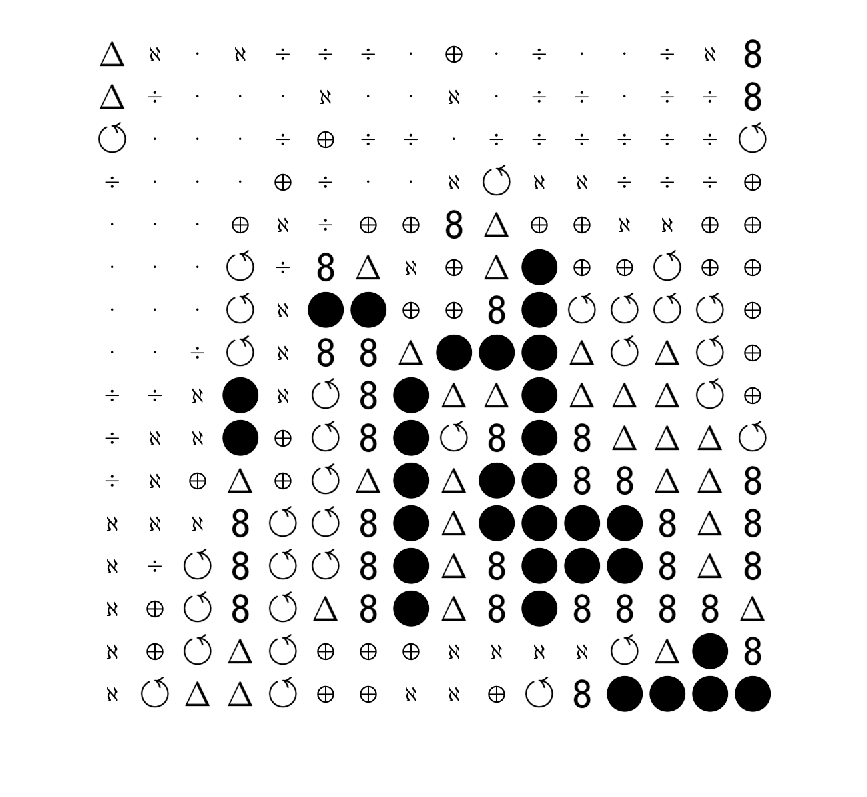
\includegraphics[width=5cm,height=5cm]{bluestreet_symbol_64.png}
		\caption{Street Symbol}
	\end{minipage}                        
\end{figure}		
\indent In the process of generating mosaics, we can obtain some information, which is shown as below.	
\begin{itemize}
	\item[-] Figure 2: runtime: 0.1563s;\; iterations: 834.
	\item[-] Figure 3: runtime: 0.0469s;\; iterations: 508.
	\item[-] Figure 5: runtime: 0.2813s;\; iterations: 1030.
	\item[-] Figure 6: runtime: 0.0313s;\; iterations: 470.
	\item[-] Figure 8: runtime: 0.1250s;\; iterations: 864.
	\item[-] Figure 9: runtime: 0.0625s;\; iterations: 504.
\end{itemize}

\indent Besides, we can get other results. All the obtained results are solutions of the original integer problem, and all the found mosaics are degenerate solutions.\\
\par Thus we can find some observations according to the above liner problems.\\
(1) When use small tiles, it will cost more time and go through more iterations to solve out the linear program; (2) The relaxation of variables will not influence the final solution;  (3) The mosaics generation problem have a high possibility to get a degenerate solution.
\thispagestyle{empty}

~\\
\normalsize \textbf{Task 2}\\ 
\par We can then derive the dual problem of the relaxed linear optimization problem. To simplify the problem, we need to change the form of the primal problem.
\begin{equation*}
\begin{aligned}
min_{\textbf{x}}\indent& c^{T}\textbf{x}\\
s.t.\indent& A\textbf{x}=b, I\textbf{x} \leqslant \bm{1}\\
& x_{i,j,k} \geqslant 0, \forall x_{i,j,k}\in \textbf{x}\\
\end{aligned}
\end{equation*}
Note that the notation $I$ is the identity matrix, and $\bm{1}$ is a column vector only contains number 1. Then we can easily formulate the dual problem.
\begin{equation*}
\begin{aligned}
max_{\textbf{y}}\indent& a^{T}\textbf{y}\\
s.t.\indent& B\textbf{y} \leqslant c\\
& y_{w} \leqslant 0, \forall w\in S\\
\end{aligned}
\end{equation*}
Note here the column vector $a =\begin{bmatrix}
b\\\bm{1}
\end{bmatrix}$, and the matrix $B =\begin{bmatrix}
A\\I
\end{bmatrix}^{T}$, and the length of set $S$ is $l =m\cdot n\cdot r$, which contains the last $l$ index of column vector $\textbf{y}$.\\

\par Then we can also use \textit{linprog} in MATLAB to solve the dual problem. The following are results of \textbf{dual} problems of corresponding figures.
\begin{itemize}
	\item[-] Figure 2: runtime: 0.3125s;\; iterations: 2643;\; duality gap: 0.
	\item[-] Figure 3: runtime: 0.1892s;\; iterations: 1153;\; duality gap: 0.
	\item[-] Figure 5: runtime: 0.2969s;\; iterations: 2860;\; duality gap: 0.
	\item[-] Figure 6: runtime: 0.1238s;\; iterations: 997;\; duality gap: 0.
	\item[-] Figure 8: runtime: 0.2500s;\; iterations: 2510;\; duality gap: 0.
	\item[-] Figure 9: runtime: 0.1875s;\; iterations: 1119;\; duality gap: 0.
\end{itemize}
\par From the above results, we can find that, in the dual problem, both of runtime and number of iterations are larger than the primal problem. Besides, we also find that, in all situations, the duality gap are all 0, which means that the optimal values in dual and primal are the same.

\thispagestyle{empty}
~\\
\normalsize \textbf{Task 3}\\
\par Up to now, we have already find mosaics for the gray-scale version of the color image $U$. We also want to include the color information in the calculation of the brightness coefficients $\beta_{i,j}$ of $U$. Then we can compute $\beta_{i,j}$ as follows.
\begin{equation*}
\beta_{i,j} = \frac{1}{3}\beta_{i,j}(red) + \frac{1}{3}\beta_{i,j}(green) + \frac{1}{3}\beta_{i,j}(blue)
\end{equation*}
Note that $\frac{1}{3}\beta_{i,j}(red)$ means the average brightness in \textbf{red} channel, $\frac{1}{3}\beta_{i,j}(green)$ means the average brightness in \textbf{green} channel, $\frac{1}{3}\beta_{i,j}(blue)$ means the average brightness in \textbf{blue} channel.\\
\par According to this method, we can get the new $\beta_{i,j}$. Since $\beta_{i.j}$ changes, then the term $(c_{k}-\beta_{i,j})^{2}$ also changes. Thus we can conduct sensitivity analysis on the primal problem.\\
\indent The new reduced cost can be checked by the following formula.
\begin{equation*}
\tilde{c}^{T}-\tilde{c}_{B}^{T}A_{B}^{-1}A \geqslant 0
\end{equation*}
where $\tilde{c}=c+\Delta c$.\\
\indent Here we treat the primal problem as a binary linear program. In order to get $\tilde{c}_{B}$ and $A_{B}$, we need to find the final basic index. Since the matrix $A$ is not of full rank, we first choose the index whose corresponding variable $x_{i,j,k}$ is equal to 1 as basic index, then we eliminate some dependent rows and columns from $A$. Thus we can get the final basic index set $B$.\\
\indent We can go through sensitivity analysis in each mosaic figures. Also, we can check the result by recomputing each linear program. Here are the results.
\begin{itemize}
	\item[-] Figure 2: exists reduced cost $c_{i} \leqslant 0$.
	\item[-] Figure 3: exists reduced cost $c_{i} \leqslant 0$.
	\item[-] Figure 5: exists reduced cost $c_{i} \leqslant 0$.
	\item[-] Figure 6: exists reduced cost $c_{i} \leqslant 0$.
	\item[-] Figure 8: exists reduced cost $c_{i} \leqslant 0$.
	\item[-] Figure 9: exists reduced cost $c_{i} \leqslant 0$.
\end{itemize}

\indent Thus we find that, in all mosaic figures, there exits some $c_{i}$ whose reduced cost is small than 0. That is, all the found mosaic figures are not still optimal for the new objective function. 

\thispagestyle{empty}
~\\
\normalsize \textbf{Task 4}\\
\par Now we can use our own tiles to generate more mosaic figures. Here we rescale the circle tiles to the size of 20*20 and symbol tiles to the size of 32*32 to generate mosaic figures.\\
\indent The following are some new mosaic figures. Figure 10-12 apply 20*20 circle tiles to generate city, street and mountain mosaics. Figure 13-15 apply 32*32 symbol tiles to generate city, street and mountain mosaics.
\newpage 
\begin{figure}[htbp]
	\centering
	\begin{minipage}[t]{0.32\linewidth}
		\centering
		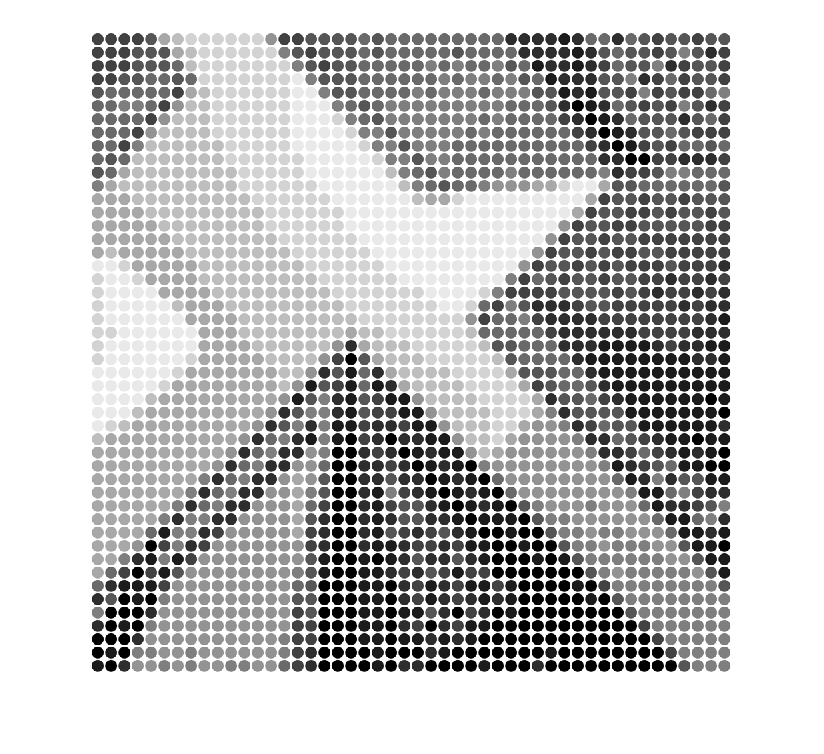
\includegraphics[width=5cm,height=5cm]{city_circle_20.png}
		\caption{City Circle}
	\end{minipage}
	\begin{minipage}[t]{0.32\linewidth}
		\centering
		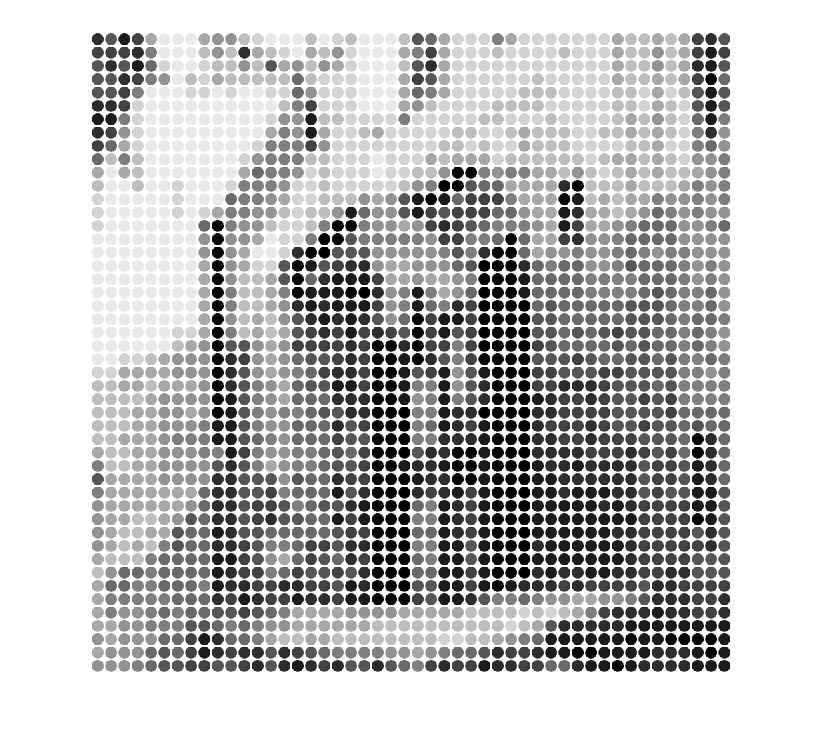
\includegraphics[width=5cm,height=5cm]{bluestreet_circle_20.png}
		\caption{Street Circle}
	\end{minipage}
	\begin{minipage}[t]{0.32\linewidth}
		\centering
		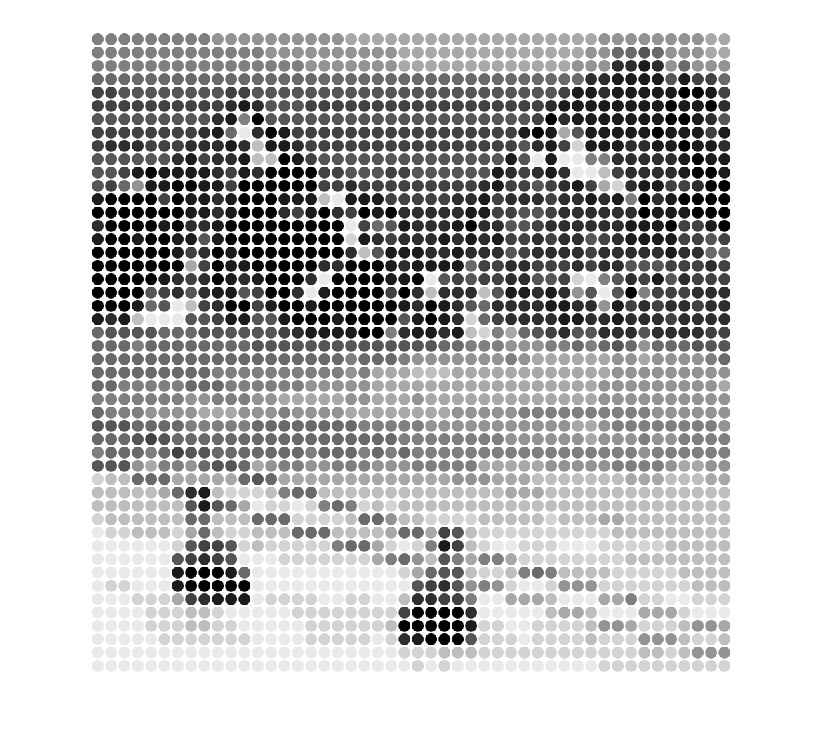
\includegraphics[width=5cm,height=5cm]{mountain_circle_20.png}
		\caption{Mountain Circle}
	\end{minipage}                        
\end{figure}

\thispagestyle{empty}
\begin{figure}[htbp]
	\centering
	\begin{minipage}[t]{0.32\linewidth}
		\centering
		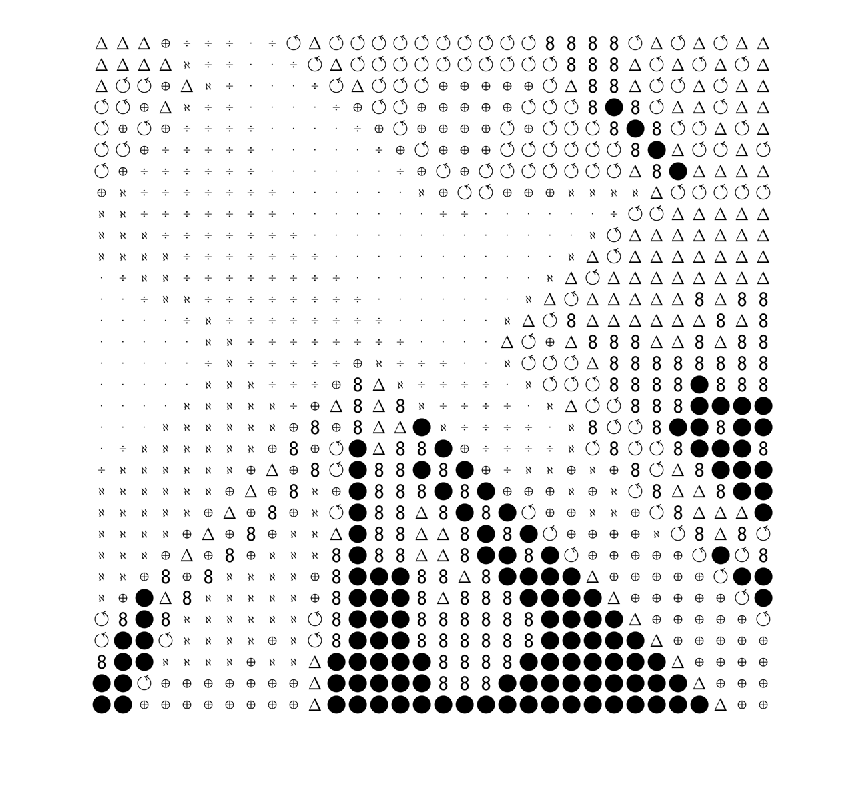
\includegraphics[width=5cm,height=5cm]{city_symbol_32.png}
		\caption{City Symbol}
	\end{minipage}
	\begin{minipage}[t]{0.32\linewidth}
		\centering
		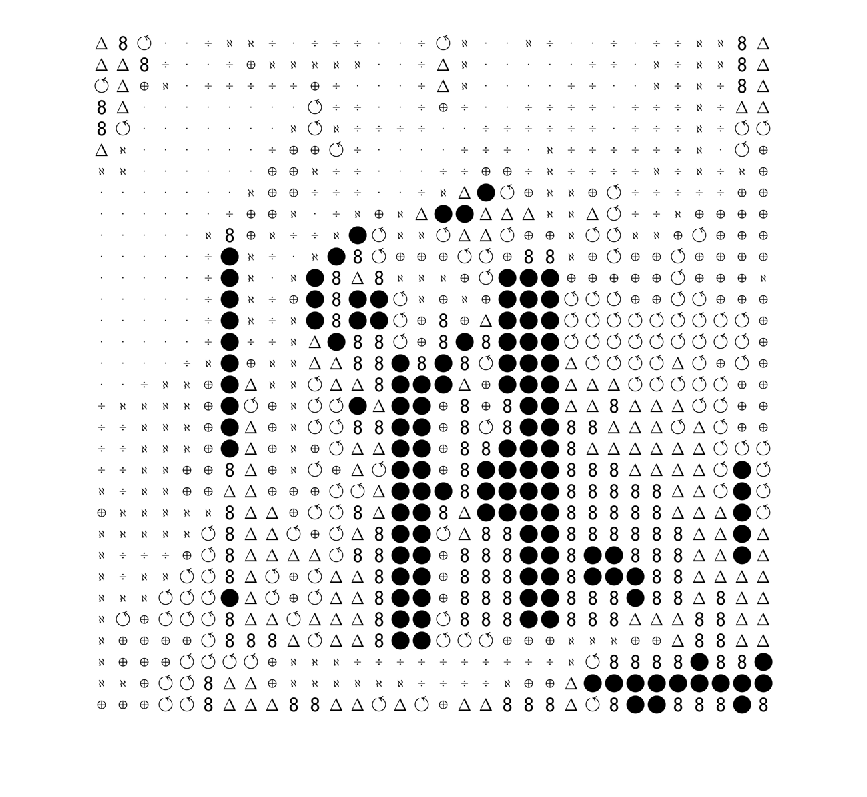
\includegraphics[width=5cm,height=5cm]{bluestreet_symbol_32.png}
		\caption{Street Symbol}
	\end{minipage}
	\begin{minipage}[t]{0.32\linewidth}
		\centering
		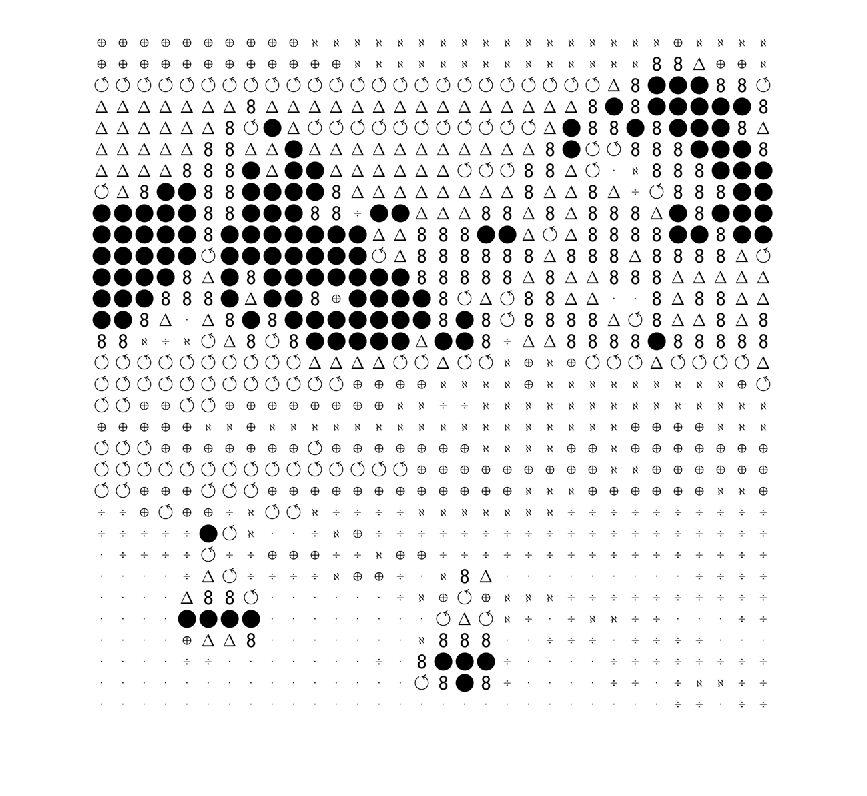
\includegraphics[width=5cm,height=5cm]{mountain_symbol_32.png}
		\caption{Mountain Symbol}
	\end{minipage}                        
\end{figure}	
	
\par What's more, we can also apply some adjustment to the original mosaic generation task. Here we want to respectively get brightness from red, green and blue channel. We can use $\beta_{i,j}(red)$, $\beta_{i,j}(green)$ and $\beta_{i,j}(blue)$ to label brightness information in each channel.\\
\indent We will solve 3 linear programs for each mosaic generation task. Besides, in order to return the closet color information in our mosaics, we relax the constraint which requires each type of tiles to be used same times. Thus we will solve the following linear programs.
\begin{equation*}
\begin{aligned}
min_{x}\indent& \sum_{k=1}^{r}\sum_{j=1}^{n}\sum_{i=1}^{m}(c_{k}-\beta_{i,j}(*))^{2}x_{i,j,k}\\
s.t.\indent& \sum_{k=1}^{r}x_{i,j,k}=1, \forall i,j\\
&  x_{i,j,k} \in \{0,1\}, \forall i,j,k
\end{aligned}
\end{equation*}
Here the label $\beta_{i,j}(*)$ can be replace by $\beta_{i,j}(red)$, $\beta_{i,j}(green)$ and $\beta_{i,j}(blue)$. After solving the linear programs, we can get 3 column vectors \textbf{x}(red), \textbf{x}(green) and \textbf{x}(blue). Then we formulate them into RGB format, thus we can get mosaic figures with color information.\\

\par The mosaic figures with color information are shown as followings, through utilizing 20*20 circle tiles used before.
\begin{figure}[htbp]
	\centering
	\begin{minipage}[t]{0.32\linewidth}
		\centering
		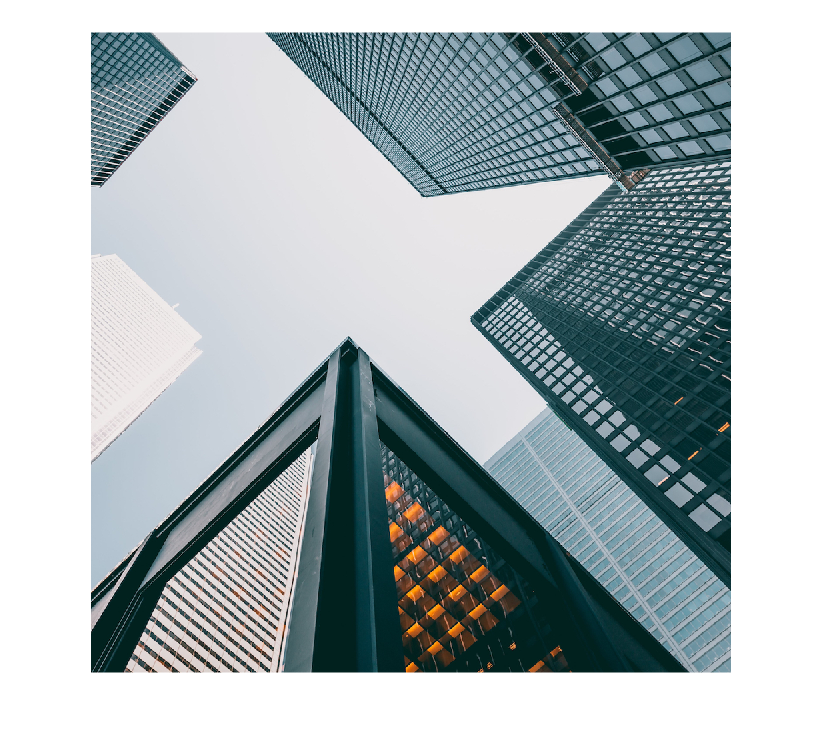
\includegraphics[width=5cm,height=5cm]{city.png}
		\caption{City RGB}
	\end{minipage}
	\begin{minipage}[t]{0.32\linewidth}
		\centering
		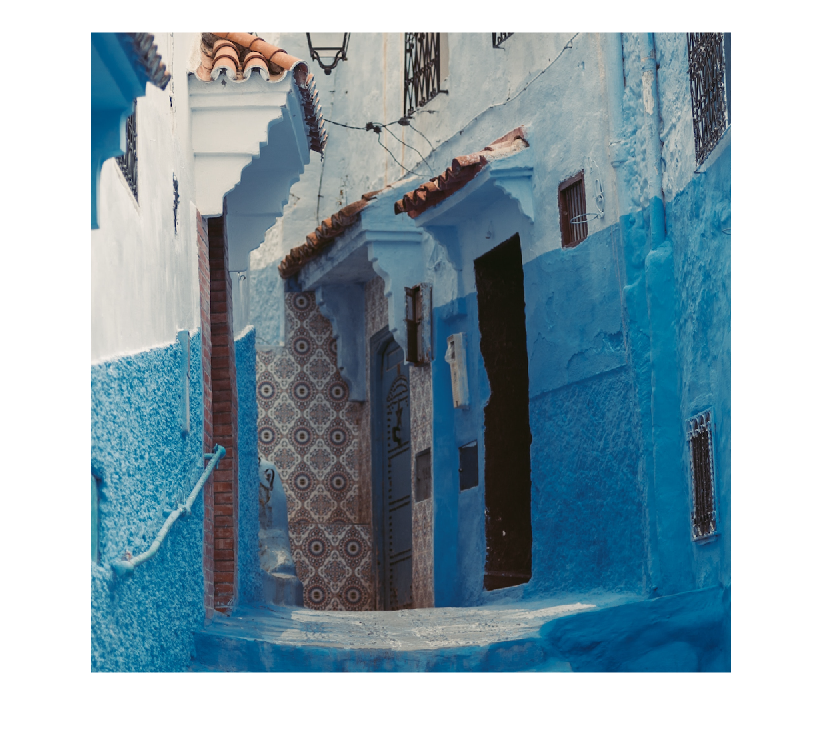
\includegraphics[width=5cm,height=5cm]{bluestreet.png}
		\caption{Street RGB}
	\end{minipage}
	\begin{minipage}[t]{0.32\linewidth}
		\centering
		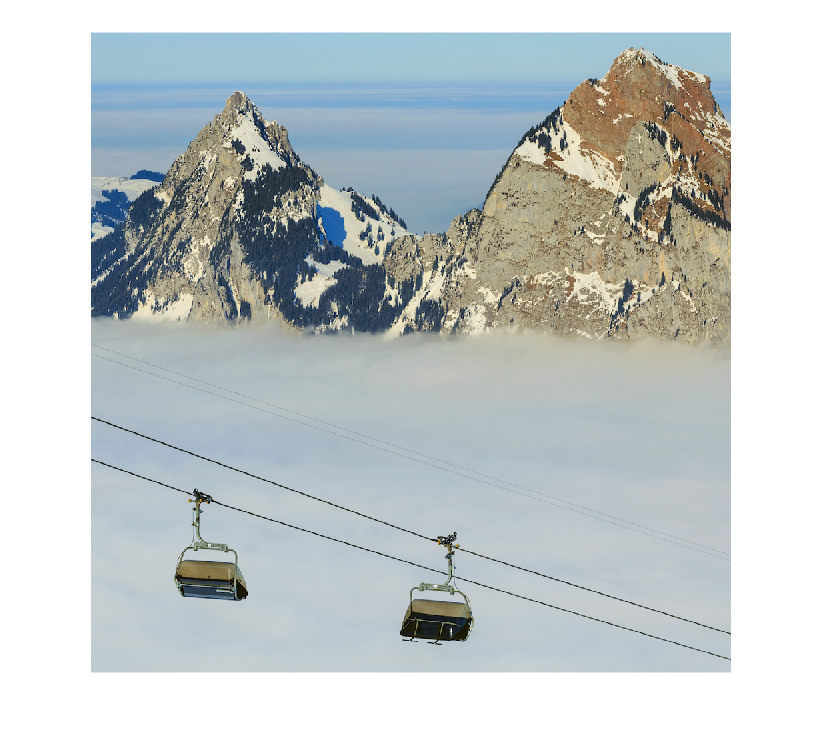
\includegraphics[width=5cm,height=5cm]{mountain.png}
		\caption{Mountain RGB}
	\end{minipage}                        
\end{figure}

\begin{figure}[htbp]
	\centering
	\begin{minipage}[t]{0.32\linewidth}
		\centering
		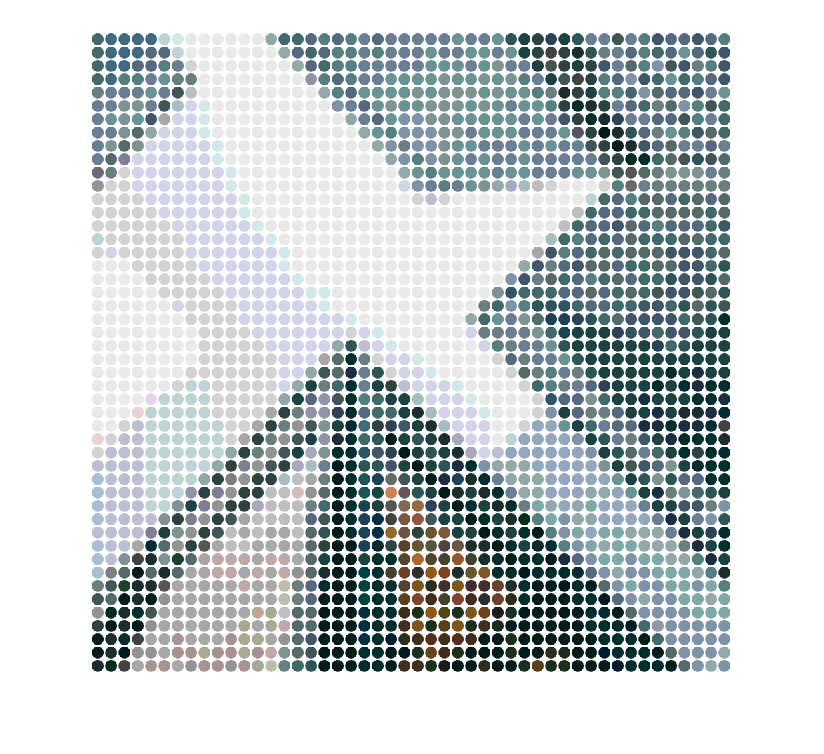
\includegraphics[width=5cm,height=5cm]{city_rgb20.png}
		\caption{City Circle}
	\end{minipage}
	\begin{minipage}[t]{0.32\linewidth}
		\centering
		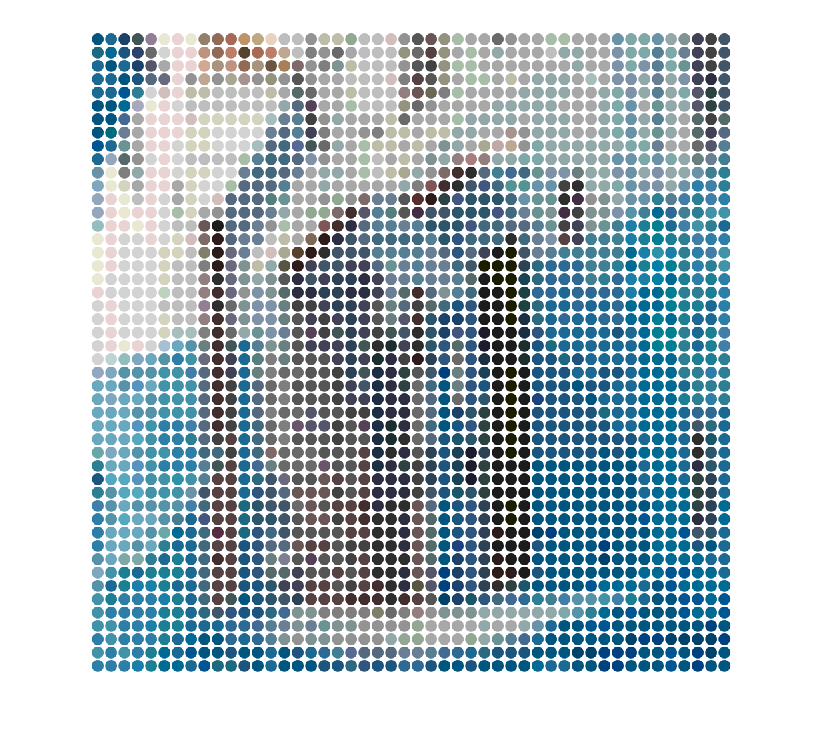
\includegraphics[width=5cm,height=5cm]{bluestreet_rgb20.png}
		\caption{Street Circle}
	\end{minipage}
	\begin{minipage}[t]{0.32\linewidth}
		\centering
		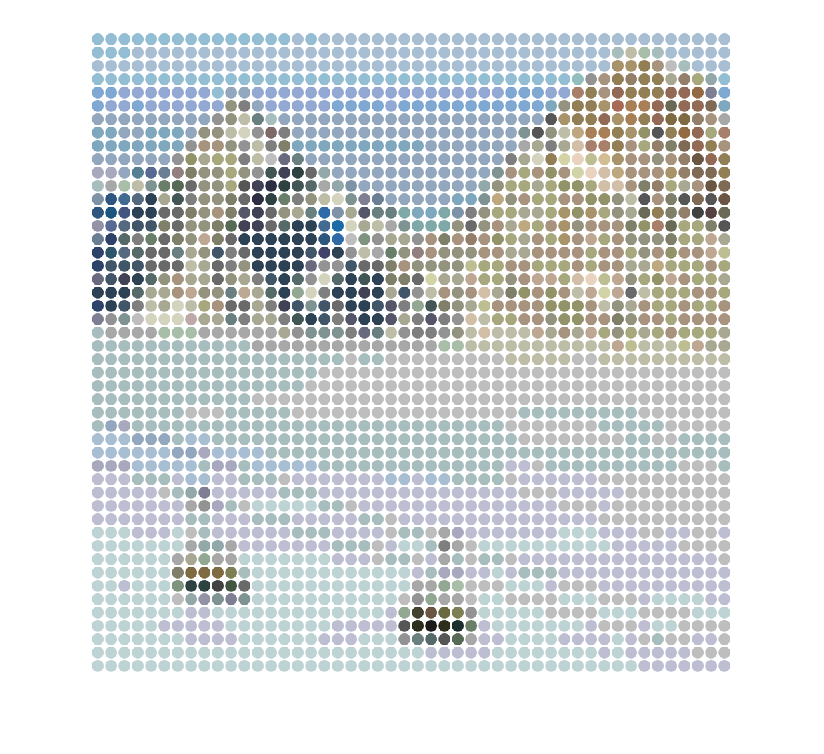
\includegraphics[width=5cm,height=5cm]{mountain_rgb20.png}
		\caption{Mountain Circle}
	\end{minipage}                        
\end{figure}
\thispagestyle{empty}
\end{document}
